\documentclass[12pt]{article}

\usepackage[T1]{fontenc}
\usepackage{amsthm}
\usepackage{amsmath}
\usepackage{amsfonts}
\usepackage[scr]{rsfso}
\usepackage{bm}
\usepackage{thmtools}
\usepackage{mathtools}
\usepackage{enumitem}
\usepackage{hyperref}
\usepackage{cancel}
\usepackage{empheq}
\usepackage{booktabs}

\usepackage{tikzit}
\input{pm.tikzstyles}

\usepackage[parfill]{parskip}
\setlength{\parindent}{0pt}
\setlength{\parskip}{2ex plus 0.2ex minus 0.2ex}

\usepackage[
paper  = letterpaper,
left   = 1in,
right  = 1in,
top    = 1in,
bottom = 1in,
]{geometry}


\newcommand{\N}{\mathbb{N}}
\newcommand{\Z}{\mathbb{Z}}
\newcommand{\Q}{\mathbb{Q}}
\newcommand{\R}{\mathbb{R}}
\newcommand{\C}{\mathbb{C}}

\newcommand{\iid}{\overset{iid}{\sim}}
\renewcommand{\Pr}{\mathbb{P}}
\newcommand{\E}{\mathbb{E}}

\newcommand{\ELBO}{\text{ELBO}}

\title{
    STCS 6701: Probabilistic Machine Learning \\
    Homework 2%
}
\author{
    Satvik Saha ({\tt ss7228})%
}
\date{
    \vspace{-1.2em}
    \today%
}

\begin{document}

\maketitle


% \tableofcontents

\section*{Problem 1}

\subsection*{Question 1.1}


\begin{enumerate}[label=(\alph*)]
    \item If $\theta_i \gg \beta_j$ and $\alpha_j > 0$, we have
    $\alpha_j(\theta_i - \beta_j) \gg 0$, hence the vote is very likely to be
    ``yea''.

    If $\theta_i$ is smaller than $\beta_j$, then $\alpha_j(\theta_i - \beta_k)
    < 0$ hence the vote is more likely to be ``nay''.


    \item Given two bills with the same $\beta_j$, the sign of $\alpha_j$
    controls the polarity of the bill.
    Fix a senator and an ideology difference $\delta := \theta_i - \beta_j$;
    a positive $\delta$ indicates that the senator is more conservative than
    the bill.
    A positive value of $\alpha_j$ makes ``yea'' more likely, while a negative
    value of $\alpha_j$ makes ``nay'' more likely; the scenario flips when
    $\delta < 0$.

    A larger magnitude of $\alpha_j$ indicates a more \emph{polarizing} bill:
    for fixed $\delta$, the mean of $z_{ij}$ is shifted further away from $0$
    as $|\alpha_j|$ becomes larger, which means that the probability of voting
    contrary to the expected direction $1(\alpha_j(\theta_i - \beta_j))$ shrinks.


    \item We need only set up our model (local latent variables $z_{ij},
    \epsilon_{ij}$) for pairs of indices $(i, j)$ for which $y_{ij}$ is
    \emph{not} missing (or held-out).
    Call the collection of all such indices $\mathscr{I}$; the joint likelihood
    for our model only contains terms from $\mathscr{I}$, and looks like \[
        p(\bm{\theta}, \bm{\alpha}, \bm{\beta}) \prod_{(i, j) \in \mathscr{I}} p(y_{ij} \mid \theta_i, \alpha_j, \beta_j).
    \] In particular, \[
        p(y_{ij} = 1\mid \theta_i, \alpha_j, \beta_j)
            = \Pr(z_{ij} > 0 \mid \theta_i, \alpha_j, \beta_j)
            = \Phi(\alpha_j(\theta_i - \beta_j)).
    \] 


    For $(i, j) \notin \mathscr{I}$, one can of course evaluate the
    posterior predictive likelihood \[
        p(y_{ij} \mid \bm{y}_{in})
            = \int p(y_{ij}\mid \theta_i, \alpha_j, \beta_j)\,p(\theta_i, \alpha_j, \beta_j \mid \bm{y}_{in})\:d\theta_i\:d\alpha_j\:d\beta_j.
    \]


    \item The model can be represented using plate notation as follows.
    \begin{center}
        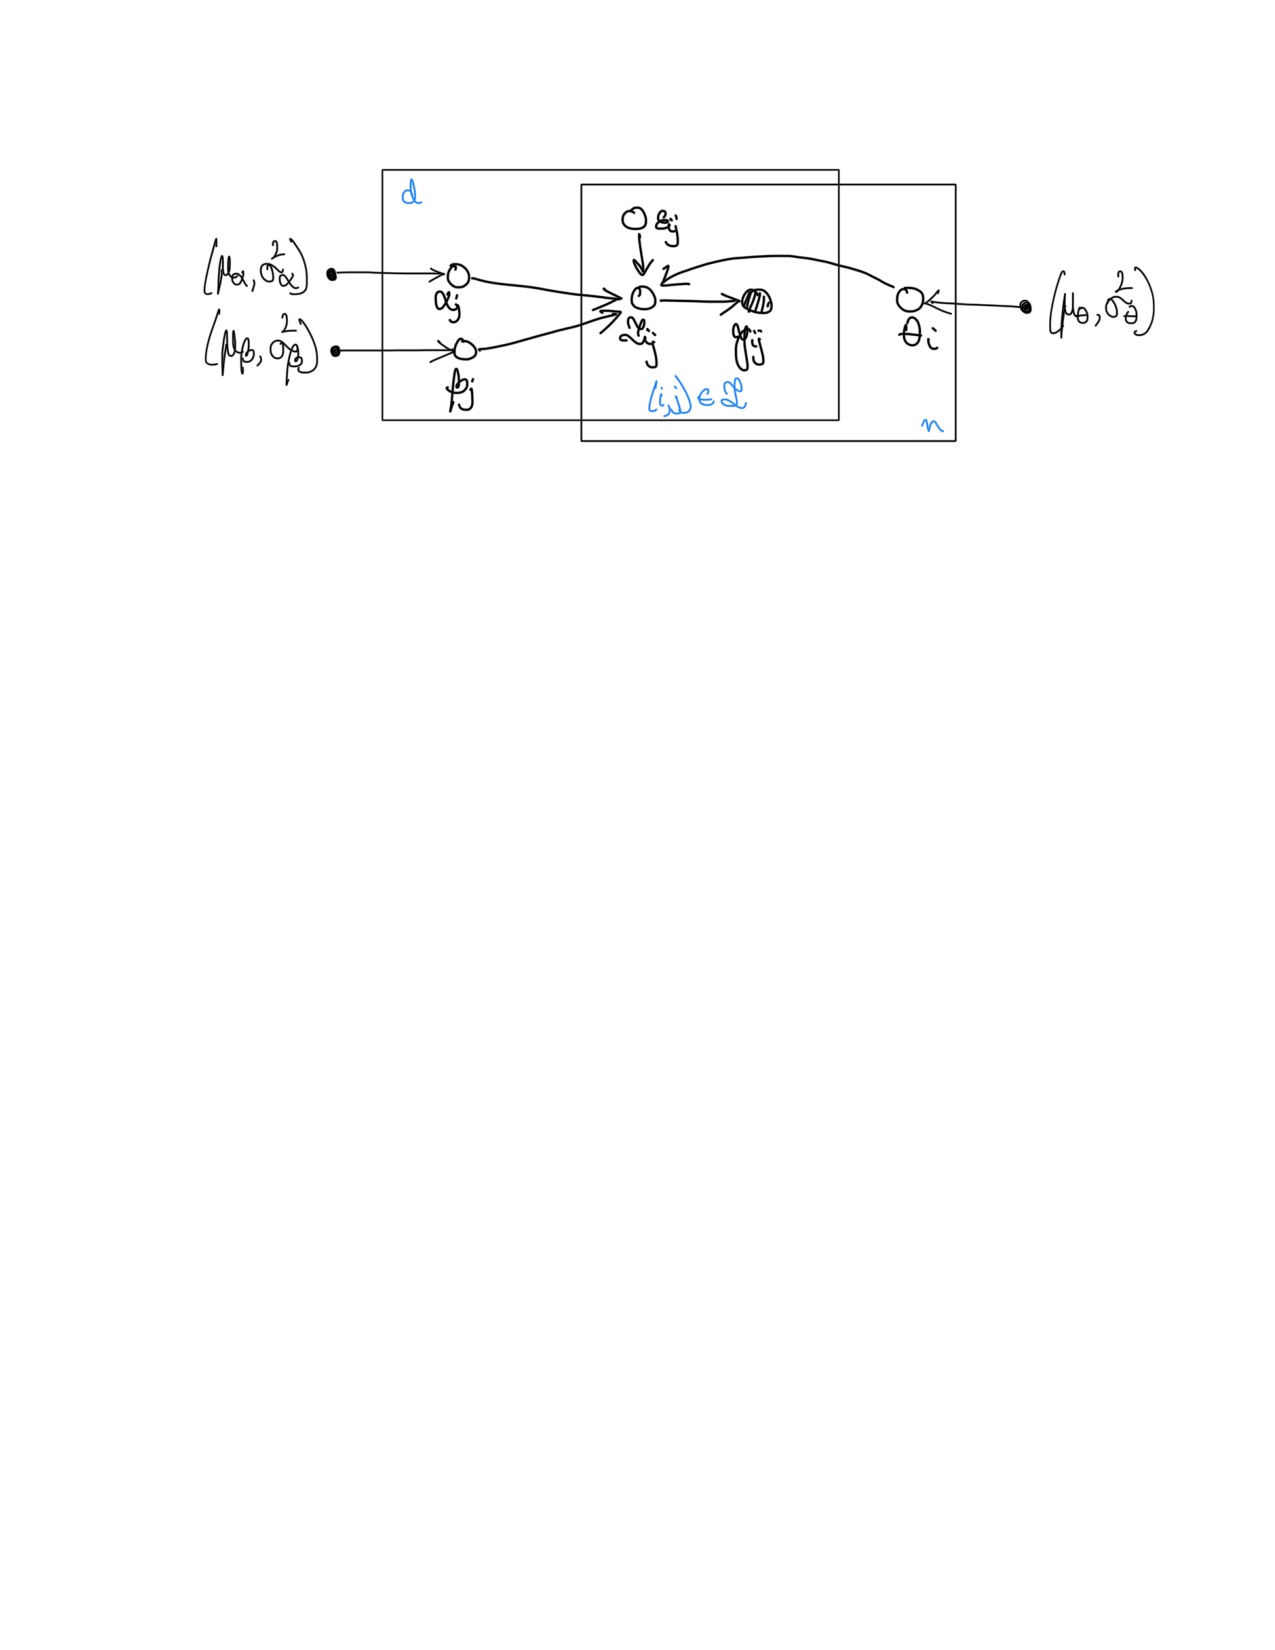
\includegraphics[width=\textwidth]{ideal_point_graphical}
    \end{center}


    \item Senator ideological positions $\theta_\cdot$ have been marked in red,
    bill positions $\beta_\cdot$ in blue on the same ideological axis.
    \begin{center}
        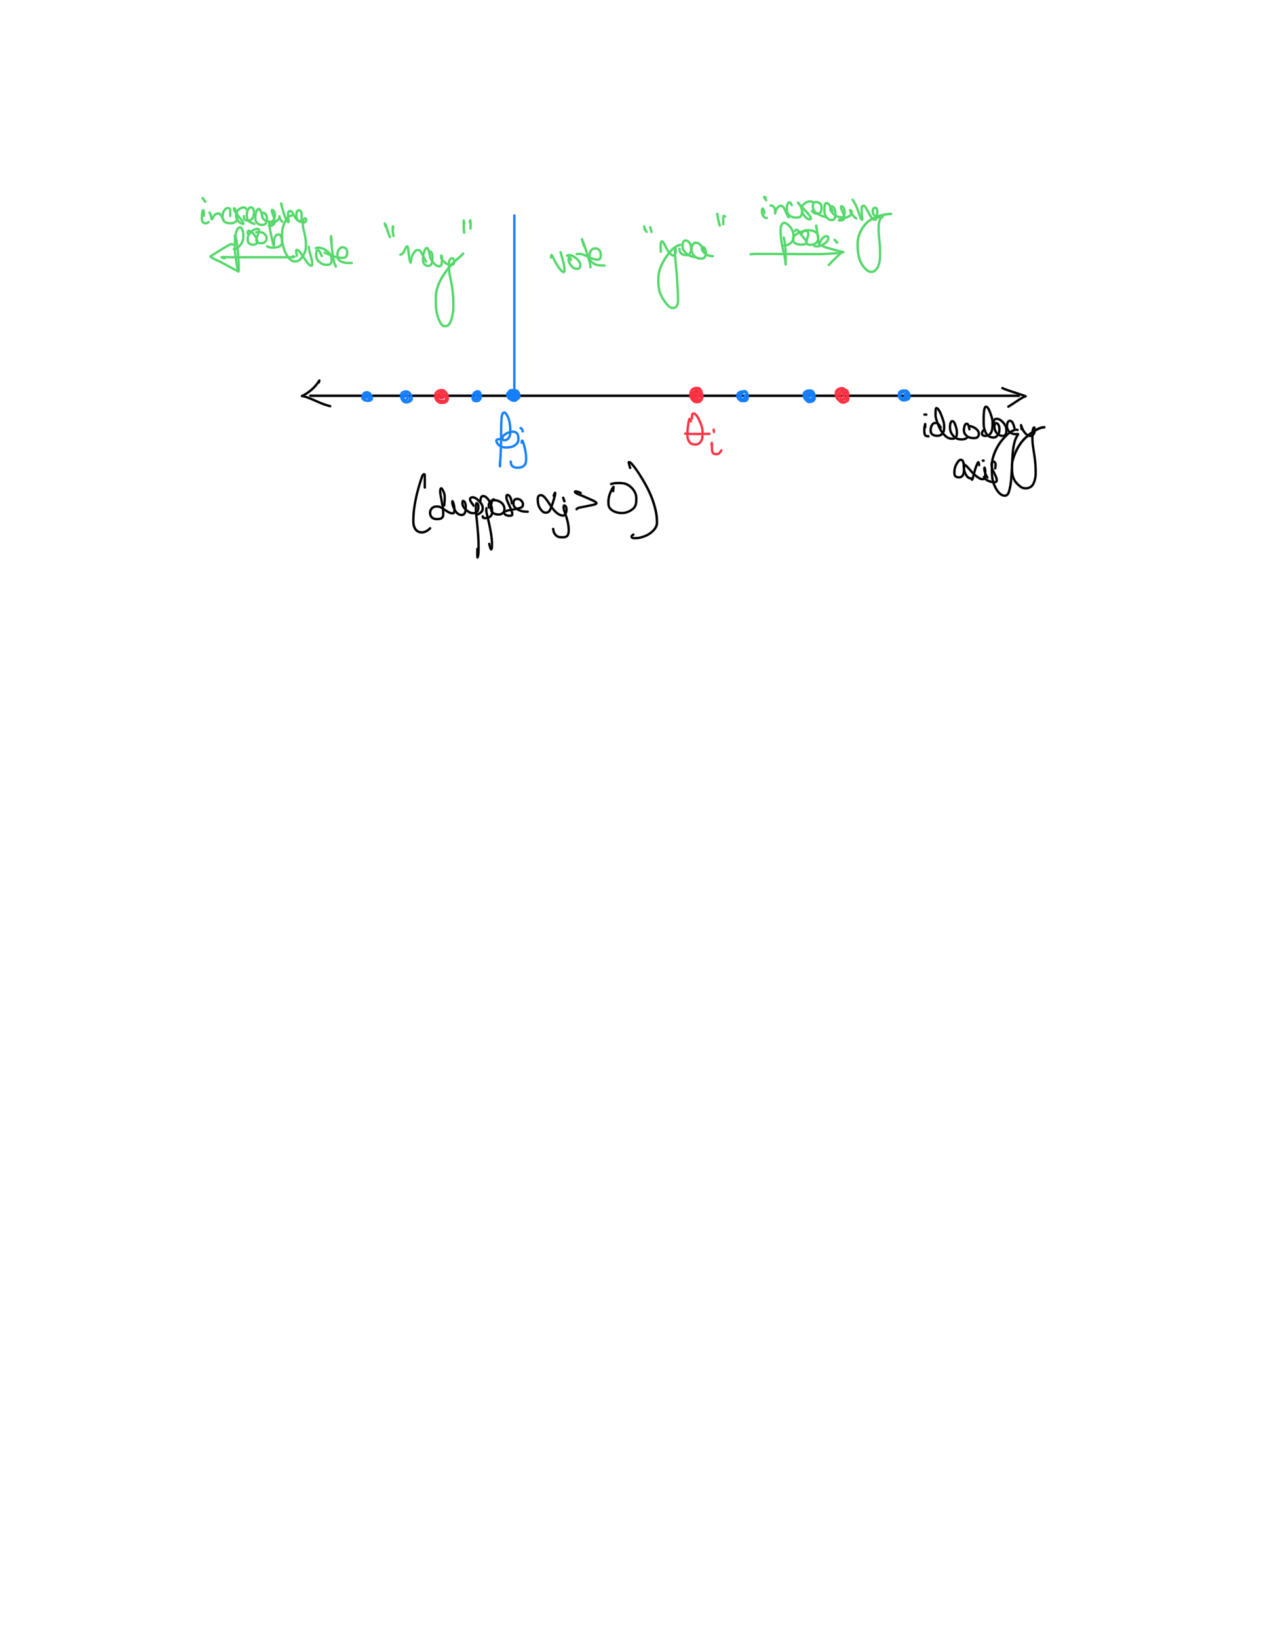
\includegraphics[width=\textwidth]{ideal_point_rule}
    \end{center}
    For the particular bill $j$, suppose that $\alpha_j > 0$ for simplicity.
    This determines a threshold: a senator $i$ with position $\theta_i >
    \beta_j$ is more likely than not to vote ``yea'', with the likelihood
    increasing the further away $\theta_\cdot$ is from the threshold.
    Conversely, senators to the left of the threshold are more likely to vote
    ``nay''.


    \item The held-out data (indexed by $\mathscr{I}_o$) can be used to compute a
    goodness of fit score, such as an average predictive log-likelihood \[
        \sum_{(i, j) \in \mathscr{I}_o} \int \log{p(y_{ij}\mid \theta_i, \alpha_j, \beta_j)}\,p(\theta_i, \alpha_j, \beta_j \mid \bm{y}_{in})\:d\theta_i\:d\alpha_j\:d\beta_j.
    \] The (approximately inferred plug-in) posterior depends on the prior
    variances; maximizing this score over choices of these prior parameters is
    an Empirical Bayes approach to setting them.
\end{enumerate}



\subsection*{Question 1.2}

\begin{enumerate}
    \item Denoting the shifted variable with accents, note that the model
    likelihood
    \begin{align*}
        \mathcal{L}(\bm{y}\mid \bm{\theta}, \bm{\alpha}, \bm{\beta})
            &= \prod_{(i, j) \in \mathscr{I}} p(y_{ij}\mid \theta_i, \alpha_j, \beta_j) \\
            &= \prod_{(i, j) \in \mathscr{I}} \Phi(\alpha_j(\theta_i - \beta_j))^{y_{ij}}(1 - \Phi(\alpha_j(\theta_i - \beta_j)))^{1 - y_{ij}}
    \end{align*}
    depends on $\bm{\theta}, \bm{\alpha}, \bm{\beta}$ only through the
    quantities $\mu_{ij} := \alpha_j(\theta_i - \beta_j)$.
    Since \[
        \alpha_j(\theta'_i - \beta'_j)
            = \alpha_j((\theta_i + c) - (\beta_j + c))
            = \alpha_j(\theta_i - \beta_j),
    \] the likelihood $\mathcal{L}$ remains unchanged after making the
    indicated replacements.

    This means that raw values on the ideological axis have no absolute
    interpretation; we may as well fix the ideological value of one item (a
    senator or a bill) and measure the ideology of all other items (senators
    and bills) relative to them.
    The model only deals with differences in ideology $\theta_i - \alpha_j$.

    \item Using the same setup, \[
        \alpha'_j(\theta'_i - \beta'_j)
            = \left(\frac{\alpha_j}{k}\right)(k\theta_i - k\beta_j)
            = \alpha_j(\theta_i - \beta_j)
    \] shows that $\mathcal{L}$ remains unchanged after making the indicated
    rescaling.

    Again, this means that the absolute scale of the ideological axis is
    arbitrary; we may as well fix the absolute value of the polarity $\alpha_j$
    of one bill (say to 1) and measure the polarities of all other bills
    relative to it.


    \item The symmetries in the parameters indicate that they can only be
    interpreted in a relative sense (differences in ideologies, ratios of
    discriminations); the raw values of these parameters are somewhat
    arbitrary.

    Combining the above symmetries shows that the model likelihood is invariant
    under the transformation \[
        \alpha_j \mapsto \alpha_j/k, \qquad
        \beta_j \mapsto k\beta_j + c, \qquad
        \theta_i \mapsto k\theta_i + c.
    \]

    The suggested choice of prior will of course break this arbitrariness,
    favoring shrinkage towards zero in the posterior.


\end{enumerate}



\subsection*{Question 1.3}

\begin{enumerate}[label=(\alph*)]
    \item Note that $y_{ij} \mid z_{ij}$ is completely determined by $1(z_{ij}
    > 0)$, with \[
        p(y_{ij}\mid z_{ij})
            = 1(z_{ij} > 0)^{y_{ij}}\,1(z_{ij} \leq 0)^{1 - y_{ij}}.
    \]
    \emph{Remark:} Here we abuse notation with $0^0 := 1$.
    This uses the interpretation $y_{ij}\mid z_{ij} \sim
    \text{Bernoulli}(1(z_{ij} > 0))$.
    More precisely, $y_{ij}\mid z_{ij} \sim \delta_{1(z_{ij} > 0)}$ since
    $y_{ij} = 1(z_{ij} > 0)$.

    Thus, the joint density is described by \begin{align*}
        p(\bm{y}, \bm{z}, \bm{\theta}, \bm{\alpha}, \bm{\beta})
            &= \prod_{i = 1}^n p(\theta_i) \prod_{j = 1}^d p(\alpha_j)\,p(\beta_j)
                \prod_{(i, j) \in \mathscr{I}} p(z_{ij}\mid \theta_i, \alpha_j, \beta_j)\,p(y_{ij}\mid z_{ij}) \\
            &= \prod_{i = 1}^n (2\pi\sigma_\theta^2)^{-1 /2} e^{-(\theta_i - \mu_\theta)^2 /2\sigma_\theta^2} \\
                &\qquad\cdot\prod_{j = 1}^d (2\pi\sigma_\alpha^2)^{-1 /2} e^{-(\alpha_j - \mu_\alpha)^2) /2\sigma_\alpha^2}\,\cdot\,
                    (2\pi\sigma_\beta^2)^{-1 /2} e^{-(\beta_j - \mu_\beta)^2) /2\sigma_\beta^2} \\
                &\qquad\cdot\prod_{(i, j) \in \mathscr{I}} (2\pi)^{-1 /2}e^{-(z_{ij} - \alpha_j(\theta_i - \beta_j))^2 / 2} \,\cdot\,
                    1(z_{ij} > 0)^{y_{ij}}\,1(z_{ij}\leq 0)^{1 - y_{ij}}. \tag{$\star$} \label{Q1_joint}
    \end{align*}
    This is zero when any $y_{ij} \neq 1(z_{ij} > 0)$, and is a product of
    Gaussian densities otherwise.


    \item Denote $\mu_{ij} = \alpha_j(\theta_i - \beta_j)$.
    Fixing all terms apart from $z_{ij}$ in the joint \eqref{Q1_joint} gives \[
        p(z_{ij} \mid -) \propto e^{-(z_{ij} - \mu_{ij})^2 /2} 1(z_{ij} > 0)^{y_{ij}} 1(z_{ij} \leq 0)^{1 - y_{ij}}.
    \] In particular, this shows \[
        p(z_{ij} \mid y_{ij}, \bm{\theta}, \bm{\alpha}, \bm{\beta}) 
            \propto e^{-(z_{ij} - \mu_{ij})^2 /2} \cdot \begin{cases}
                1(z_{ij} > 0), &\text{ if } y_{ij} = 1, \\
                1(z_{ij} \leq 0), &\text{ if } y_{ij} = 0,
            \end{cases}
    \] which means that \[
        z_{ij} \mid y_{ij}, \bm{\theta}, \bm{\alpha}, \bm{\beta} \sim \begin{cases}
            N(\mu_{ij}, 1)\text{ truncated to }(0, \infty), &\text{ if } y_{ij} = 1, \\
            N(\mu_{ij}, 1)\text{ truncated to }(-\infty, 0], &\text{ if } y_{ij} = 0.
        \end{cases}
    \]

    This assumes that $(i, j) \in \mathscr{I}$, i.e.\ that $y_{ij}$ was observed.
    If not, $y_{ij}$ is not part of our model (does not appear in the joint
    distribution), so there is no question of a corresponding $z_{ij}$
    appearing anywhere.


    \item Fixing all terms apart from $\theta_i$ in the joint density of
    $(\bm{z}, \bm{\theta}, \bm{\alpha}, \bm{\beta})$ (obtained by simply
    dropping $\bm{y}$ from the generative process described by
    \eqref{Q1_joint}) gives \[
        p(\theta_i \mid \bm{z}, \bm{\alpha}, \bm{\beta})
            \propto e^{-(\theta_i - \mu_\theta)^2 /2\sigma_\theta^2}
                \prod_{j: (i, j) \in \mathscr{I}} e^{-(z_{ij} - \alpha_j(\theta_i - \beta_j))^2 / 2}.
    \] The logarithm of this density is a negative definite quadratic in
    $\theta_i$, hence this must describe a Gaussian $N(\mu_{\theta_i},
    \sigma_{\theta_i}^2)$.
    In particular, the logarithm of the above expression is \begin{align*}
        h(\theta_i)
            &:= -\frac{1}{2\sigma_\theta^2} (\theta_i - \mu_\theta)^2 -\frac{1}{2}\sum_{j: (i, j) \in \mathscr{I}} (z_{ij} - \alpha_j(\theta_i - \beta_j))^2 \\
            &=: -\frac{1}{2\sigma_{\theta_i}^2}(\theta_i - \mu_{\theta_i})^2 + C(\bm{z}, \bm{\alpha}, \bm{\beta}).
    \end{align*}
    Then, \begin{align*}
        -h'(\theta_i)
            = \frac{1}{\sigma_\theta^2} (\theta_i - \mu_\theta) -\sum_{j: (i, j) \in \mathscr{I}} \alpha_j (z_{ij} - \alpha_j(\theta_i - \beta_j))
            = \frac{1}{\sigma_{\theta_i}^2}(\theta_i - \mu_{\theta_i}),
    \end{align*}
    so comparing coefficients gives the parameters \[
        \sigma_{\theta_i}^{-2} = \sigma_{\theta}^{-2} + \sum_{j: (i, j) \in \mathscr{I}} \alpha_j^2, \qquad
        \mu_{\theta_i} = \sigma_{\theta_i}^2\left(\sigma_{\theta}^{-2}\mu_{\theta} + \sum_{j: (i, j) \in \mathscr{I}} \alpha_j(z_{ij} + \alpha_j\beta_j)\right).
    \]


    \item Repeating the same arguments from above on $\beta_j$, we have \[
        p(\beta_j \mid \bm{z}, \bm{\theta}, \bm{\alpha})
            \propto e^{-(\beta_j - \mu_\beta)^2 / 2\sigma_\beta^2} \prod_{i: (i, j) \in \mathscr{I}} e^{-(z_{ij} - \alpha_j(\theta_i - \beta_j))^2 / 2}.
    \] Again, the log-density is a negative definite quadratic in $\beta_j$,
    hence this describes a Gaussian $N(\mu_{\beta_j}, \sigma_{\beta_j}^2)$.
    Calling the logarithm of the above expression $h(\beta_j)$, we match \[
        -h'(\beta_j)
            = \frac{1}{\sigma_\beta^2}(\beta_j - \mu_\beta) + \sum_{i: (i, j) \in \mathscr{I}} \alpha_j(z_{ij} - \alpha_j(\theta_i - \beta_j))
            =: \frac{1}{\sigma_{\beta_j}^2}(\beta_j - \mu_{\beta_j}),
    \] so comparing coefficients gives \[
        \sigma_{\beta_j}^{-2} = \sigma_{\beta}^{-2} + \sum_{i: (i, j) \in \mathscr{I}} \alpha_j^2, \qquad
        \mu_{\beta_j} = \sigma_{\beta_j}^2\left(\sigma_{\beta}^{-2}\mu_\beta - \sum_{i: (i, j) \in \mathscr{I}} \alpha_j(z_{ij} - \alpha_j\theta_i)\right).
    \] 


    \item Repeating the same arguments from above on $\alpha_j$, we have \[
        p(\alpha_j \mid \bm{z}, \bm{\theta}, \bm{\beta})
            \propto e^{-(\alpha_j - \mu_\alpha)^2 / 2\sigma_\alpha^2} \prod_{i: (i, j) \in \mathscr{I}} e^{-(z_{ij} - \alpha_j(\theta_i - \beta_j))^2 / 2}.
    \] Again, the log-density is a negative definite quadratic in $\alpha_j$,
    hence describes a Gaussian $N(\mu_{\alpha_j}, \sigma_{\alpha_j}^2)$.
    Calling the logarithm of the above expression $h(\alpha_j)$, we match \[
        -h'(\alpha_j)
            = \frac{1}{\sigma_\alpha^2}(\alpha_j - \mu_\alpha) - \sum_{i: (i, j) \in \mathscr{I}} (\theta_i - \beta_j)(z_{ij} - \alpha_j(\theta_i - \beta_j))
            =: \frac{1}{\sigma_{\alpha_j}^2}(\alpha_j - \mu_{\alpha_j}),
    \] so comparing coefficients gives \[
        \sigma_{\alpha_j}^{-2} = \sigma_{\alpha}^{-2} + \sum_{i: (i, j) \in \mathscr{I}} (\theta_i - \beta_j)^2, \qquad
        \mu_{\alpha_j} = \sigma_{\alpha_j}^2\left(\sigma_{\alpha}^{-2}\mu_\alpha + \sum_{i: (i, j) \in \mathscr{I}} (\theta_i - \beta_j)z_{ij}\right).
    \] 

    \item We have already computed \[
        y_{ij} \mid \bm{\theta}, \bm{\alpha}, \bm{\beta}
            \sim \text{Bernoulli}(\Phi(\mu_{ij})),
    \] and the `collapsed' likelihood $p(\bm{y}\mid\bm{\theta}, \bm{\alpha},
    \bm{\beta})$ in Q1.2.1.
    Restating this here, \[
        p(\bm{y} \mid \bm{\theta}, \bm{\alpha}, \bm{\beta})
            = \prod_{(i, j) \in \mathscr{I}} \Phi(\mu_{ij})^{y_{ij}} (1 - \Phi(\mu_{ij}))^{1 - y_{ij}},
    \] hence \begin{align*}
        p(\bm{y}, \bm{\theta}, \bm{\alpha}, \bm{\beta})
            &= \prod_{i = 1}^n (2\pi\sigma_\theta^2)^{-1 /2} e^{-(\theta_i - \mu_\theta)^2 /2\sigma_\theta^2} \\
                &\qquad\cdot\prod_{j = 1}^d (2\pi\sigma_\alpha^2)^{-1 /2} e^{-(\alpha_j - \mu_\alpha)^2) /2\sigma_\alpha^2}\,\cdot\,
                    (2\pi\sigma_\beta^2)^{-1 /2} e^{-(\beta_j - \mu_\beta)^2) /2\sigma_\beta^2} \\
                &\qquad\cdot\prod_{(i, j) \in \mathscr{I}} \Phi(\mu_{ij})^{y_{ij}} (1 - \Phi(\mu_{ij}))^{1 - y_{ij}}.
    \end{align*}


    \item Our variational family is described by \begin{align*}
        q(\theta_i) &\sim N(\bar{\mu}_{\theta_i}, \bar{\sigma}_{\theta_i}^2), \quad& 1 \leq i \leq n, \\
        q(\alpha_j) &\sim N(\bar{\mu}_{\alpha_j}, \bar{\sigma}_{\alpha_j}^2), & 1 \leq j \leq d, \\
        q(\beta_j) &\sim N(\bar{\mu}_{\beta_j}, \bar{\sigma}_{\beta_j}^2), & 1 \leq j \leq d, \\
        q(z_{ij}) &\sim N(\bar{\mu}_{ij}, 1) \text{ truncated to } \begin{cases}
            (0, \infty), &\text{ if } y_{ij} = 1, \\
            (-\infty, 0], &\text{ if } y_{ij} = 0,
        \end{cases} &(i, j) \in \mathscr{I}.
    \end{align*}

    Each update will require the $q$-expectation of the log densities
    (discarding `constants' not involving the parameter being updated) of the
    full-conditionals which we have computed in parts (b)-(e).
    Thus, the updates for \begin{itemize}
        \item $q(z_{ij})$ require $\E_q[\mu_{ij}] = \E_q[\alpha_j](\E_q[\theta_i] - \E_q[\beta_j])$,
        \item $q(\theta_i)$ require $\E_q[z_{ij}]$, $\E_q[\beta_j]$, $\E_q[\alpha_j]$, $\E_q[\alpha_j^2]$,
        \item $q(\alpha_j)$ require $\E_q[z_{ij}]$, $\E_q[\theta_i]$, $\E_q[\theta_i^2]$, $\E_q[\beta_j]$, $\E_q[\beta_j^2]$,
        \item $q(\beta_j)$ require $\E_q[z_{ij}]$, $\E_q[\theta_i]$, $\E_q[\alpha_j]$, $\E_q[\alpha_j^2]$.
    \end{itemize}



    \item \begin{enumerate}[label=(\roman*)]
        \item Reusing our work from part (b), the log-density of the
        full-conditional of $z_{ij}$ is quadratic (restricted to $\R_{\pm}$
        based on $y_{ij}$) in $z_{ij}$ with coefficients $-\frac{1}{2}$ and
        $\mu_{ij}$.
        Taking expectations, we obtain $\bar{\mu}_{ij} = \E_q[\mu_{ij}] =
        \bar{\mu}_{\alpha_j}(\bar{\mu}_{\theta_i} - \bar{\mu}_{\beta_j})$.

        With this, \[
            \E_q[z_{ij}] = \bar{\mu}_{ij} + \phi(\bar{\mu}_{ij})\cdot \begin{cases}
                1 /\Phi(\bar{\mu}_{ij}), &\text{ if } y_{ij} = 1, \\
                -1 / (1 - \Phi(\bar{\mu}_{ij})), &\text{ if } y_{ij} = 0.
            \end{cases}
        \]


        \item Reusing our work from part (c), the log-density of the
        full-conditional of $\theta_i$ is quadratic in $\theta_i$; taking
        expectations and comparing coefficients on the $\theta_i$-derivative of
        the log density again (these operations commute!), we have \[
            \bar{\sigma}_{\theta_i}^{-2} = \sigma_{\theta}^{-2} + \sum_{j: (i, j) \in \mathscr{I}} \E_q[\alpha_j^2], \quad
            \bar{\mu}_{\theta_i} = \bar{\sigma}_{\theta_i}^2\left(\sigma_\theta^{-2}\mu_\theta + \sum_{j: (i, j) \in \mathscr{I}} (\E_q[\alpha_j]\E_q[z_{ij}] + \E_q[\alpha_j^2]\E_q[\beta_j])\right).
        \] Applying precisely the same arguments on the full-conditional of
        $\beta_j$ gives the updates \[
            \bar{\sigma}_{\beta_j}^{-2} = \sigma_{\beta}^{-2} + \sum_{i: (i, j) \in \mathscr{I}} \E_q[\alpha_j^2], \quad
            \bar{\mu}_{\beta_j} = \bar{\sigma}_{\beta_j}^2\left(\sigma_{\beta}^{-2}\mu_\beta - \sum_{i: (i, j) \in \mathscr{I}} (\E_q[\alpha_j]\E_q[z_{ij}] - \E_q[\alpha_j^2]\E_q[\theta_i])\right).
        \] 

        \item Repeating the same arguments on the full-conditional density of
        $\alpha_j$ gives the updates \[
            \bar{\sigma}_{\alpha_j}^{-2} = \sigma_{\alpha}^{-2} + \sum_{i: (i, j) \in \mathscr{I}} \E_q[(\theta_i - \beta_j)^2], \quad
            \bar{\mu}_{\alpha_j} = \bar{\sigma}_{\alpha_j}^2\left(\sigma_{\alpha}^{-2}\mu_\alpha + \sum_{i: (i, j) \in \mathscr{I}} (\E_q[\theta_i] - \E_q[\beta_j])\E_q[z_{ij}]\right).
        \] Note that \[
            \E_q[(\theta_i - \beta_j)^2] = \E_q[\theta_i^2] + \E_q[\beta_j^2] - 2\E_q[\theta_i]\E_q[\beta_j].
        \] 
    \end{enumerate}

\end{enumerate}


\clearpage

\begin{center}
{\LARGE
    Probit Ideal Point Modeling for Voting Patterns
}
\end{center}
\vspace{2em}

\begin{abstract}
    We apply a probit ideal point model on a dataset of roll-call votes from
    the 113th U.S.\ Senate to model voting patterns, and reveal latent
    ideological structures inherent to both senators and bills.
    Approximate inference is performed using a Coordinate Ascent Variational
    Inference (CAVI) algorithm.
    The inferred ideologies are easily interpretable as degrees of political
    left/right inclination.
\end{abstract}
\vspace{1em}


\subsection*{Introduction}

Voting patterns in the U.S.\ Senate are determined by political ideology.
An ideal point model quantifies this latent ideology for both senators and
bills on a one-dimensional scale, with the difference between a senator's
ideological position and the bill's location monotonically affecting the
probability of voting ``yea''.
We analyze the 113th U.S.\ Senate roll-call votes using a probit ideal point
model, and observe that the inferred ideological axis is consistent with
senators' party affiliation and left/right wing political inclination.
This supports the conclusion that voting patterns are largely driven by the
latter factors.
The results have been presented in Figure~\ref{fig:ideal_points} for senators,
Figure~\ref{fig:bill_landscape} for bills.

\begin{figure}[h!]
\begin{center}
    \vspace{1em}
    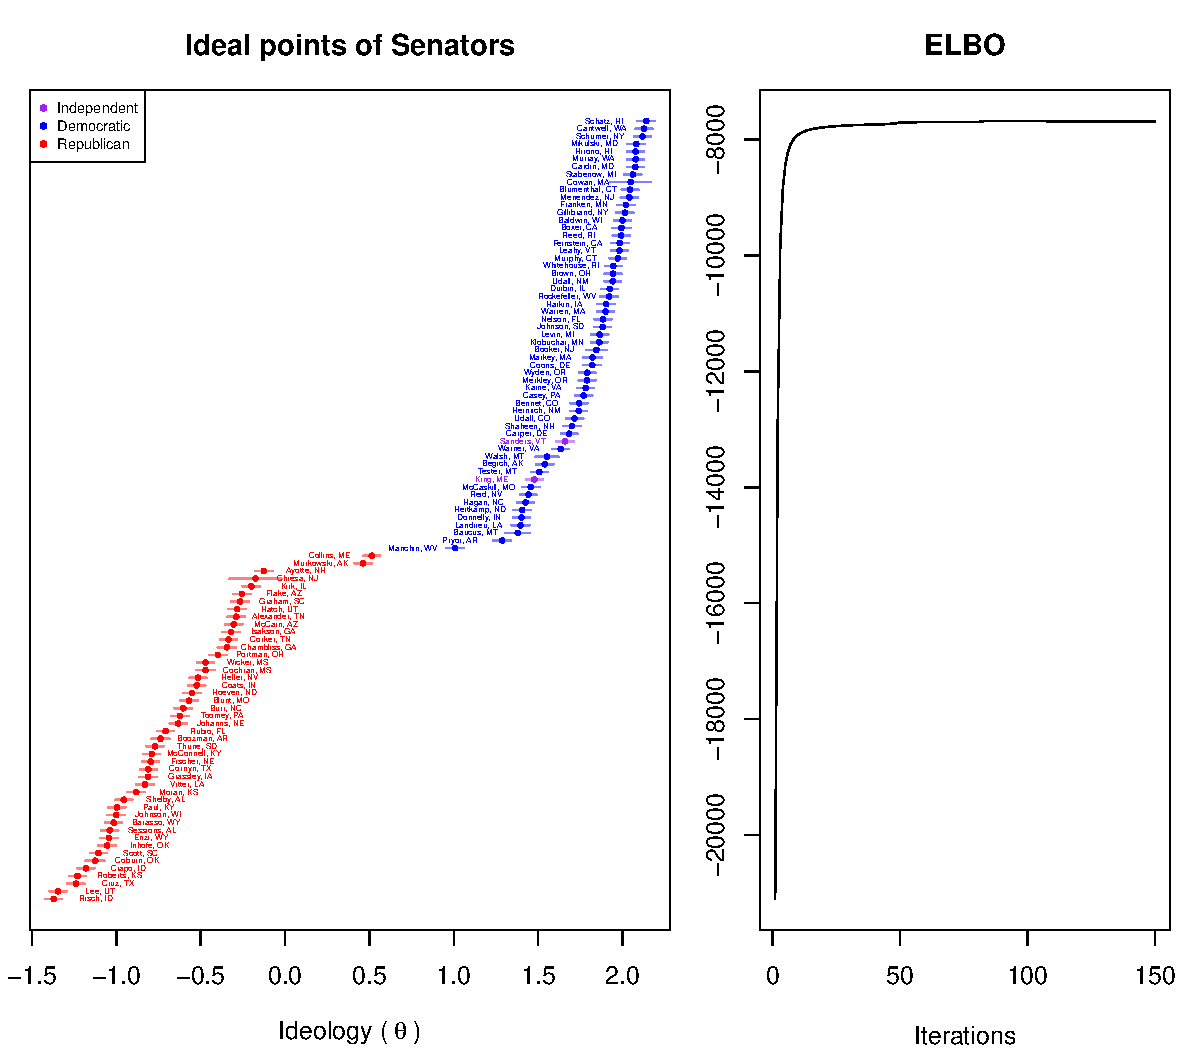
\includegraphics[width=\textwidth]{ideal_points_elbo}
\end{center}
\caption{
    \emph{Left:} Approximate posterior ideologies of senators, depicted as
    $\bar{\mu}_{\theta_i} \pm 2\bar{\sigma}_{\theta_i}$.
    This is consistent with party affiliation, denoted by color.
    The large error bars on Cowan, Chiesa correspond to the unusually small
    number of votes they cast (154, 70).
    \emph{Right:} Evolution of the ELBO of the mean-field variational posterior
    $q_\nu$ over iterations.
}
\label{fig:ideal_points}
\end{figure}


\subsection*{Model}

Fix $n, d \in \N$, and let $\mathscr{I} \subseteq \{1, \dots, n\} \times \{1,
\dots, d\}$ be the collection of pairs $(i, j)$ for which the $i$-th senator
has voted on the $j$-th bill.
Setting prior parameters $\mu_\theta, \mu_\alpha, \mu_\beta \in \R$,
$\sigma_\theta^2, \sigma_\alpha^2, \sigma_\beta^2 \in \R^+$, and denoting
$\mu_{ij} := \alpha_j (\theta_i - \beta_j)$, consider the following generative
model.
\begin{align*}
    \theta_i &\sim \text{Normal}(\mu_\theta, \sigma_\theta^2), &1 \leq i \leq n, \\
    \alpha_j &\sim \text{Normal}(\mu_\alpha, \sigma_\alpha^2), &1 \leq j \leq d, \\
    \beta_j  &\sim \text{Normal}(\mu_\beta,  \sigma_\beta^2),  &1 \leq j \leq d, \\
    z_{ij} \mid \theta_i, \alpha_j, \beta_j &\sim \text{Normal}(\mu_{ij}, 1), &(i, j) \in \mathscr{I} \\
    y_{ij} \mid z_{ij} &= 1(z_{ij} > 0), &(i, j) \in \mathscr{I}.
\end{align*}

Abusing notation with $0^0 := 1$, the joint density of this model is
\begin{align*}
    p(\bm{y}, \bm{z}, \bm{\theta}, \bm{\alpha}, \bm{\beta})
        &= \prod_{i = 1}^n (2\pi\sigma_\theta^2)^{-1 /2} e^{-(\theta_i - \mu_\theta)^2 /2\sigma_\theta^2} \\
            &\qquad\cdot\prod_{j = 1}^d (2\pi\sigma_\alpha^2)^{-1 /2} e^{-(\alpha_j - \mu_\alpha)^2) /2\sigma_\alpha^2}\,\cdot\,
                (2\pi\sigma_\beta^2)^{-1 /2} e^{-(\beta_j - \mu_\beta)^2) /2\sigma_\beta^2} \\
            &\qquad\cdot\prod_{(i, j) \in \mathscr{I}} (2\pi)^{-1 /2}e^{-(z_{ij} - \alpha_j(\theta_i - \beta_j))^2 / 2} \,\cdot\,
                1(z_{ij} > 0)^{y_{ij}}\,1(z_{ij}\leq 0)^{1 - y_{ij}}.
\end{align*}
This is zero when any $y_{ij} \neq 1(z_{ij} > 0)$, and is a product of
Gaussian densities otherwise.

Each senator's ideological position $\theta_i$ interacts with a bill's
ideological threshold $\beta_j$ and polarizing power $\alpha_j$ to give the
likelihood $\Phi(\alpha_j(\theta_i - \beta_j))$ of a vote ``yea'' in the pair
$(i, j)$.


\subsection*{Inference}

We use Mean-Field Variational Inference with a Coordinate Ascent Variational
Inference (CAVI) algorithm to approximate the posterior distribution of
$\bm{z}, \bm{\theta}, \bm{\alpha}, \bm{\beta} \mid \bm{y}$.
We use a variational family \[
    q_\nu(\bm{z}, \bm{\theta}, \bm{\alpha}, \bm{\beta})
        = \prod_{i = 1}^n q(\theta_i; \bar{\mu}_{\theta_i}, \bar{\sigma}_{\theta_i}^2)
            \prod_{j = 1}^d q(\alpha_j; \bar{\mu}_{\alpha_j}, \bar{\sigma}_{\alpha_j}^2)\,
                q(\beta_j; \bar{\mu}_{\beta_j}, \bar{\sigma}_{\beta_j}^2)
            \prod_{(i, j) \in \mathscr{I}} q(z_{ij}; \bar{\mu}_{ij})
\] parametrized by \[
    \nu := (
        \{\bar{\mu}_{\theta_i}\}_{i = 1}^n, \{\bar{\sigma}_{\theta_i}^2\}_{i = 1}^n,
        \{\bar{\mu}_{\alpha_j}\}_{j = 1}^d, \{\bar{\sigma}_{\alpha_j}^2\}_{j = 1}^d,
        \{\bar{\mu}_{\beta_j}\}_{j = 1}^d, \{\bar{\sigma}_{\beta_j}^2\}_{j = 1}^d,
        \{\bar{\mu}_{ij}\}_{(i, j) \in \mathscr{I}}
    ),
\] where \begin{align*}
    q(\theta_i) &\sim N(\bar{\mu}_{\theta_i}, \bar{\sigma}_{\theta_i}^2), \quad& 1 \leq i \leq n, \\
    q(\alpha_j) &\sim N(\bar{\mu}_{\alpha_j}, \bar{\sigma}_{\alpha_j}^2), & 1 \leq j \leq d, \\
    q(\beta_j) &\sim N(\bar{\mu}_{\beta_j}, \bar{\sigma}_{\beta_j}^2), & 1 \leq j \leq d, \\
    q(z_{ij}) &\sim N(\bar{\mu}_{ij}, 1) \text{ truncated to } \begin{cases}
        (0, \infty), &\text{ if } y_{ij} = 1, \\
        (-\infty, 0], &\text{ if } y_{ij} = 0,
    \end{cases} &(i, j) \in \mathscr{I}.
\end{align*}

This implies the coordinate-wise updates (to be applied in succession)
\begin{align*}
        \bar{\mu}_{ij}
            &= \bar{\mu}_{\alpha_j}(\bar{\mu}_{\theta_i} - \bar{\mu}_{\beta_j}), \\
        \bar{\sigma}_{\theta_i}^{-2}
            &= \sigma_{\theta}^{-2} + \sum_{j: (i, j) \in \mathscr{I}} (\bar{\mu}_{\alpha_j}^2 + \bar{\sigma}_{\alpha_j}^2), \\
        \bar{\mu}_{\theta_i}
            &= \bar{\sigma}_{\theta_i}^2\left(\sigma_\theta^{-2}\mu_\theta + \sum_{j: (i, j) \in \mathscr{I}} (\bar{\mu}_{\alpha_j}\E_q[z_{ij}] + (\bar{\mu}_{\alpha_j}^2 + \bar{\sigma}_{\alpha_j}^2)\bar{\mu}_{\beta_j})\right) \\
        \bar{\sigma}_{\beta_j}^{-2}
            &= \sigma_{\beta}^{-2} + \sum_{i: (i, j) \in \mathscr{I}} (\bar{\mu}_{\alpha_j}^2 + \bar{\sigma}_{\alpha_j}^2), \\
        \bar{\mu}_{\beta_j}
            &= \bar{\sigma}_{\beta_j}^2\left(\sigma_{\beta}^{-2}\mu_\beta - \sum_{i: (i, j) \in \mathscr{I}} (\bar{\mu}_{\alpha_j}\E_q[z_{ij}] - (\bar{\mu}_{\alpha_j}^2 + \bar{\sigma}_{\alpha_j}^2)\bar{\mu}_{\theta_i})\right) \\
        \bar{\sigma}_{\alpha_j}^{-2}
            &= \sigma_{\alpha}^{-2} + \sum_{i: (i, j) \in \mathscr{I}} (\bar{\mu}_{\theta_i}^2 + \bar{\sigma}_{\theta_i}^2 + \bar{\mu}_{\beta_j}^2 + \bar{\sigma}_{\beta_j}^2 - 2\bar{\mu}_{\theta_i}\bar{\mu}_{\beta_j}), \\
        \bar{\mu}_{\alpha_j}
            &= \bar{\sigma}_{\alpha_j}^2\left(\sigma_{\alpha}^{-2}\mu_\alpha + \sum_{i: (i, j) \in \mathscr{I}} (\bar{\mu}_{\theta_i} - \bar{\mu}_{\beta_j})\E_q[z_{ij}]\right).
\end{align*}
Here, \[
    \E_q[z_{ij}] = \bar{\mu}_{ij} + \phi(\bar{\mu}_{ij})\cdot \begin{cases}
        1 /\Phi(\bar{\mu}_{ij}), &\text{ if } y_{ij} = 1, \\
        -1 / (1 - \Phi(\bar{\mu}_{ij})), &\text{ if } y_{ij} = 0.
    \end{cases}
\] 

The Evidence Lower Bound (ELBO) can be directly computed as \begin{align*}
    \ELBO(q_\nu)
        &:= \E_q[\log{p(\bm{y}, \bm{z}, \bm{\theta}, \bm{\alpha}, \bm{\beta})} - \log{q(\bm{z}, \bm{\theta}, \bm{\alpha}, \bm{\beta})}] \\
        &\overset{c}{=} \frac{1}{2}\sum_{i = 1}^n \left(\log{\frac{\bar{\sigma}_{\theta_i}^2}{\sigma_{\theta}^2}} + 1 - \frac{\bar{\sigma}_{\theta_i}^2}{\sigma_\theta^2} - \frac{(\bar{\mu}_{\theta_i} - \mu_{\theta})^2}{\sigma_\theta^2}\right) \\
            &\quad + \frac{1}{2}\sum_{j = 1}^d \left(\log{\frac{\bar{\sigma}_{\alpha_j}^2}{\sigma_{\alpha}^2}} + 1 - \frac{\bar{\sigma}_{\alpha_j}^2}{\sigma_\alpha^2} - \frac{(\bar{\mu}_{\alpha_j} - \mu_{\alpha})^2}{\sigma_\alpha^2}\right) \\
            &\quad + \frac{1}{2}\sum_{j = 1}^d \left(\log{\frac{\bar{\sigma}_{\beta_j}^2}{\sigma_{\beta}^2}} + 1 - \frac{\bar{\sigma}_{\beta_j}^2}{\sigma_\beta^2} - \frac{(\bar{\mu}_{\beta_j} - \mu_{\beta})^2}{\sigma_\beta^2}\right) \\
            &\quad + \frac{1}{2}\sum_{(i, j) \in \mathscr{I}} \left(2\E_q[z_{ij}] - \mu_{ij} - \bar{\mu}_{ij}\right)(\mu_{ij} - \bar{\mu}_{ij}).
\end{align*}
The last equality is up to constants that do not depend on the variational
parameters $\nu$.


\begin{figure}[h!]
\begin{center}
    \vspace{1em}
    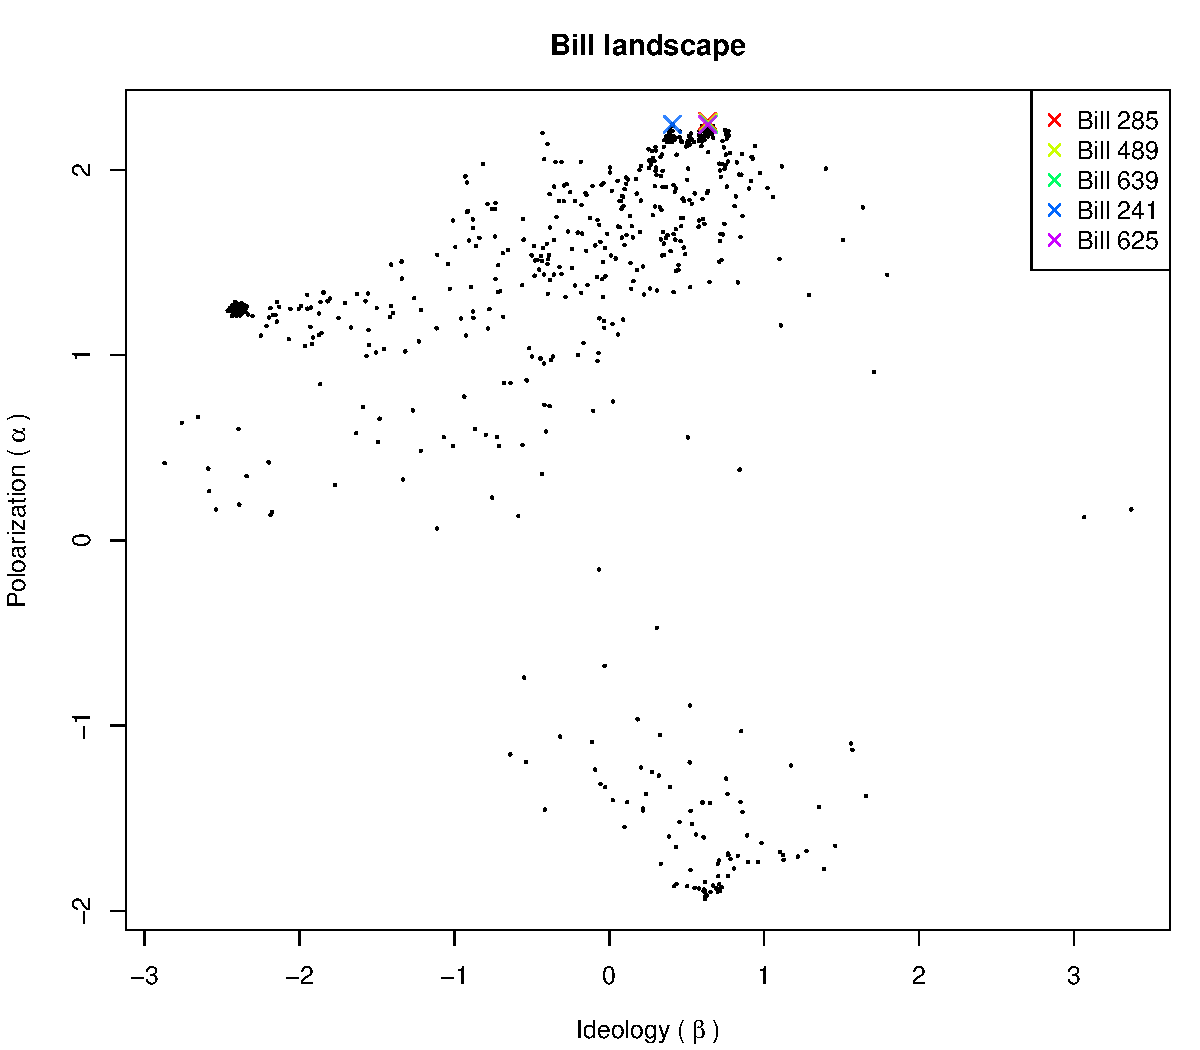
\includegraphics[width=\textwidth]{bill_landscape}
\end{center}
\caption{
    Approximate posterior ideological thresholds and polarizing powers of
    bills, depicted as $(\bar\mu_{\beta_j}, \bar\mu_{\alpha_j})$.
    The five most polarizing bills (with largest estimated magnitude of
    $\alpha_j$) have been annotated.
}
\label{fig:bill_landscape}
\end{figure}



\subsection*{Data and setup}

Votes $\bm{y}$ from $n = 103$ senators across $d = 657$ bills are recorded,
with $|\mathscr{I}| = 63254$ actual votes cast.
We set $10\%$ of these votes aside for model validation.
Each $y_{ij} \in \{0, 1\}$ for $(i, j) \in \mathscr{I}$ indicates a vote ``nay'' or
``yea'' respectively by senator $i$ on bill $j$.

When fitting our model, we choose prior hyperparameters $\mu_{\theta} =
\mu_{\beta} = 0$, $\mu_{\alpha} = 1$, $\sigma_\theta^2 = \sigma_\beta^2 =
\sigma_\alpha^2 = 1$, with the understanding that the sheer amount of data will
make a precise tuning of these weakly informative priors largely redundant.
The prior on $\bm{\alpha}$ largely determines the scale of the ideological
axis, and is somewhat arbitrary.


\subsection*{Results}

We summarize the variational posteriors $q(\theta_i; \bar{\mu}_{\theta_i},
\bar{\sigma}_{\theta_i}^2)$ of the senator ideologies in
Figure.~\ref{fig:ideal_points} (left).
The means $\bar{\mu}_{\theta_i}$ are used to rank senators in order of
left/right political inclination; the observed split aligns cleanly with party
affiliations.
The ideological positions of the 2 Independent senators seem to lean largely
towards those of the Democratic party.
As expected, the uncertainty in the posterior of $\theta_i$ is generally
inversely related to the number of votes cast by senator $i$: see Cowan, Chiesa.

The bill landscape has been summarized in Figure~\ref{fig:bill_landscape}, with
the five most polarizing bills marked.
Their ideological positions $\beta_j$ seem to fall right on the line separating
the Republican and Democratic senators.
The main bulk of bills seem to fall to the left of this threshold and with
positive $\alpha_j$, indicating that it is likely that almost all Democratic
senators (with larger ideological position $\beta_i$) would have viewed them
favorably.


\subsection*{Diagnostics}

The ELBO stabilizes within $\approx100$ iterations after a sharp monotonic
increase (Figure~\ref{fig:ideal_points}, right), which gives some measure of
confidence that CAVI updates have found a good maximum.
Qualitatively, the fitted model produces sensible interpretable results.

Evaluating the fitted model on the held-out set, $\{y_{ij}\}_{(i, j) \in
\mathscr{I}_o}$ yields a prediction accuracy of 94.4\%, and an average log
posterior predictive density score of $-0.144$.
A prediction for $y_{ij}$ is obtained by rounding the posterior
predictive probability \[
    \Pr(y_{ij} = 1 \mid \bm{y}_\text{in})
        = \int \Phi(\alpha_j(\theta_i - \beta_j))\,p(\theta_i, \alpha_j, \beta_j \mid \bm{y}_{in})\:d\theta_i\:d\alpha_j\:d\beta_j,
\] which in turn is approximated as a Monte-Carlo average over samples of
$(\theta_i, \alpha_j, \beta_j)$ from $q_{\nu^*}$.
The posterior variances seem small enough that plugging in the point estimates
$(\bar\mu_{\theta_i}, \bar\mu_{\alpha_j}, \bar\mu_{\beta_j})$ ought to give a
decent estimate, $\Phi(\bar\mu_{\alpha_j}(\bar\mu_{\theta_i} -
\bar\mu_{\beta_j}))$.



\clearpage

\section*{Question 4}


Image segmentation generally describes the process of separating an image into
different groups or regions of pixels, with pixels in a group sharing
similar characteristics..
A crude method of image segmentation involves clustering pixels by their color,
with no regard to their spatial arrangement.
In this work, we explore simple ways of introducing spatial structure to a mixture
model for segmenting color images; this is accomplished by imposing suitable
priors on group labels.
In particular, we focus on hierarchical Potts-Markov-like priors which
encourage smoothing based on neighborhoods and group-specific temperatures.
We further derive corresponding mean-field variational inference procedures and
apply this method on the Berkeley Segmentation Dataset.




\end{document}
